\documentclass[11pt,a4paper]{article}
\usepackage[utf8]{inputenc}
\usepackage[T1]{fontenc}
\usepackage{amsmath,amssymb,amsfonts,amsthm}
\usepackage{graphicx}
\usepackage{subcaption}
\usepackage{booktabs}
\usepackage{tabularx}
\usepackage{geometry}
\usepackage{hyperref}
\usepackage[most]{tcolorbox}

\geometry{top=2.2cm,bottom=2.2cm,left=2.2cm,right=2.2cm}
\graphicspath{{plots/}}

\hypersetup{
    colorlinks=true,
    linkcolor=blue!70!black,
    citecolor=blue!70!black,
    urlcolor=blue!70!black
}

\title{\textbf{Dynamical Systems Formulation of Local PCA Dimension\\and Attractor Curvature Artifacts in Müller--Israel--Stewart Theory}}
\author{\textbf{Antigravity QGP Collaboration}}
\date{\today}

\begin{document}
\maketitle

\begin{abstract}
We present a complete, closed-form dynamical systems derivation connecting the macroscopic equations of relativistic hydrodynamics to the empirical local intrinsic dimension estimated via Local Principal Component Analysis (LPCA) and the Participation Ratio (PR). Working in logarithmic state coordinates $\mathbf{x} = (\ln(T/T_0), \mathcal{A})^T$ and logarithmic proper time $t = \ln(\tau/\tau_0)$, we linearize the conformal Müller--Israel--Stewart (MIS) equations of motion around the universal hydrodynamic attractor. The resulting $2\times 2$ Jacobian matrix $\mathbf{J}$ exhibits a clean spectral separation: a marginal eigenvalue $\mu_1 \approx 0$ whose eigenvector is tangent to the attractor curve, and a fast non-hydrodynamic eigenvalue $\mu_2 \approx -\gamma(w) < 0$ ($\gamma \equiv w / C_{\tau_\pi} \gg 1$) oriented along the pressure anisotropy axis. We prove that the local covariance tensor $\mathbf{\Sigma}(t)$ contracts with an exponential damping rate of $2\gamma$, yielding an analytical participation ratio trajectory $d_{\mathrm{PR}}(t) = (1 + e^{-2\gamma t})^2 / (1 + e^{-4\gamma t}) \approx 1 + 2e^{-2\gamma t}$. Furthermore, we resolve the microscopic origin of the neighborhood parameter $k$: along a curved attractor $\mathcal{A}_{\mathrm{attr}}$, the geometric sagitta of an arc segment of length $L \propto k/N$ injects an extrinsic normal variance $\lambda_2(k) = \frac{1}{720}\kappa_{\mathrm{F}}^2 L^4$, producing a quadratic curvature bias $\lambda_2/\lambda_1 = \frac{1}{60}\kappa_{\mathrm{F}}^2 L^2 \propto \kappa_{\mathrm{F}}^2 (k/N)^2$. We validate these theoretical scalings against high-statistics numerical simulations ($N = 10\,000$ trajectories), demonstrating that $Z$-score standardization preserves scale and chart invariance, while the trade-off between Marchenko--Pastur spectral noise ($\sim 1/k$) and curvature sagitta ($\sim k^2$) dictates the optimal neighborhood size $K_{\mathrm{opt}} \sim N^{0.45}\sqrt{D}$.
\end{abstract}

\vspace{0.5em}
\tableofcontents
\newpage

% ==============================================================================
\section{Introduction and Dynamical State Representation}
\label{sec:dynamical_state}
% ==============================================================================
In relativistic heavy-ion collisions, the early non-equilibrium expansion of the Quark-Gluon Plasma (QGP) is characterized by a rapid collapse of phase-space degrees of freedom onto a low-dimensional manifold known as the \emph{hydrodynamic attractor} \cite{Heller2015,Romatschke2017,Spalinski2016}. To diagnose this hydrodynamization process quantitatively without imposing model-dependent thresholds, recent studies employ Local Principal Component Analysis (LPCA) and the continuous Participation Ratio (PR) dimension \cite{Campadelli2015,LittleMaggioni2009}:
\begin{equation}
    d_{\mathrm{PR}} = \frac{\left(\mathrm{Tr}\,\mathbf{\Sigma}\right)^2}{\mathrm{Tr}\left(\mathbf{\Sigma}^2\right)} = \frac{\left(\lambda_1 + \lambda_2\right)^2}{\lambda_1^2 + \lambda_2^2},
    \label{eq:d_pr_definition}
\end{equation}
where $\lambda_1, \lambda_2$ are the eigenvalues of the empirical local covariance matrix $\mathbf{\Sigma} \in \mathbb{R}^{2 \times 2}$ constructed from the $k$ nearest neighbors of a given state.

While LPCA is traditionally formulated within the abstract language of Riemannian submanifolds, the underlying point cloud is physically generated by a system of autonomous differential equations. Here, we build an exact bridge between the macroscopic hydrodynamic equations of motion and the microscopic spectral properties of $\mathbf{\Sigma}$.

\subsection{State Vector and Dimensionless Time}
Consider Bjorken 1D boost-invariant conformal expansion. Let $\tau_0$ and $T_0$ denote reference proper time and temperature scales. We define the dimensionless logarithmic time $t$ and state vector $\mathbf{x}(t) \in \mathbb{R}^2$:
\begin{equation}
    t \equiv \ln\left(\frac{\tau}{\tau_0}\right), \qquad \frac{d}{dt} = \tau \frac{d}{d\tau},
\end{equation}
\begin{equation}
    \mathbf{x}(t) = \begin{pmatrix} x_1(t) \\ x_2(t) \end{pmatrix} \equiv \begin{pmatrix} \ln\left(\frac{T(t)}{T_0}\right) \\ \mathcal{A}(t) \end{pmatrix},
    \label{eq:state_vector}
\end{equation}
where $x_1$ represents the logarithmic temperature and $x_2 \equiv \mathcal{A} \equiv (\mathcal{P}_T - \mathcal{P}_L)/\mathcal{P} = -6\Pi/\mathcal{E}$ is the dimensionless pressure anisotropy.

\subsection{Phase Velocity Field}
The conformal Müller--Israel--Stewart (MIS) equations of motion define the autonomous phase velocity vector $\mathbf{v}(\mathbf{x}) = \frac{d\mathbf{x}}{dt}$:
\begin{equation}
    \frac{d\mathbf{x}}{dt} = \mathbf{v}(\mathbf{x}) = \begin{pmatrix} v_1(x_1, x_2) \\ v_2(x_1, x_2) \end{pmatrix}.
\end{equation}
From energy-momentum conservation ($\partial_\mu T^{\mu\nu} = 0$), the Bjorken cooling law is exact for conformal fluids:
\begin{equation}
    \tau \frac{dT}{d\tau} = T \left(-\frac{1}{3} + \frac{\mathcal{A}}{18}\right) \implies v_1(x_1, x_2) = -\frac{1}{3}\left(1 - \frac{x_2}{6}\right).
    \label{eq:v1_definition}
\end{equation}
Notice that $v_1$ depends exclusively on the anisotropy $x_2$ and is entirely independent of $x_1$.

For the anisotropy evolution, the conformal MIS equation reads:
\begin{equation}
    \tau \frac{d\mathcal{A}}{d\tau} = \frac{1}{C_{\tau_\pi}} \left[ 8 C_\eta - w \mathcal{A} - \frac{2}{9} C_{\tau_\pi} \mathcal{A}^2 \right],
    \label{eq:v2_exact}
\end{equation}
where $C_\eta = \eta/s$, $C_{\tau_\pi} = \tau_\pi T = \mathrm{const}$, and $w \equiv \tau T = \tau_0 T_0 e^{t + x_1}$. 

Linearizing around the universal attractor curve $\mathcal{A}_{\mathrm{attr}}(w)$, the velocity component $v_2$ governs rapid relaxation toward the attractor:
\begin{equation}
    v_2(x_1, x_2) \approx -\gamma(w)\big(x_2 - \mathcal{A}_{\mathrm{attr}}(w)\big),
    \label{eq:v2_linearized}
\end{equation}
where the dimensionless damping coefficient satisfies:
\begin{equation}
    \gamma(w) \equiv \frac{w}{C_{\tau_\pi}} = \frac{\tau}{\tau_\pi(T)} \gg 1.
\end{equation}
In typical QGP conditions ($\tau \ge 0.2\,\mathrm{fm}/c, T \ge 300\,\mathrm{MeV}$), $w \gtrsim 0.6$ and $C_{\tau_\pi} \approx 0.208$, yielding $\gamma(w) \approx 3$--$15 \gg 1$.

% ==============================================================================
\section{Evolution of a Local Point Cloud: The Jacobian Matrix \texorpdfstring{$\mathbf{J}$}{J}}
\label{sec:jacobian_matrix}
% ==============================================================================
Let $\mathbf{x}_0(t)$ denote a reference trajectory on or near the attractor, and let $\mathbf{x}(t) = \mathbf{x}_0(t) + \delta\mathbf{x}(t)$ describe a nearby neighbor within a local cloud. The displacement vector $\delta\mathbf{x}(t) = (\delta x_1, \delta x_2)^T$ obeys the linearized variational equation:
\begin{equation}
    \frac{d}{dt} \begin{pmatrix} \delta x_1 \\ \delta x_2 \end{pmatrix} = \mathbf{J} \begin{pmatrix} \delta x_1 \\ \delta x_2 \end{pmatrix},
    \label{eq:variational_eq}
\end{equation}
where $\mathbf{J} \in \mathbb{R}^{2 \times 2}$ is the Jacobian matrix evaluated along $\mathbf{x}_0$:
\begin{equation}
    \mathbf{J} = \begin{pmatrix} 
    \frac{\partial v_1}{\partial x_1} & \frac{\partial v_1}{\partial x_2} \\[0.5em]
    \frac{\partial v_2}{\partial x_1} & \frac{\partial v_2}{\partial x_2} 
    \end{pmatrix}.
\end{equation}

\subsection{Matrix Elements}
Evaluating the partial derivatives directly from Eqs.~(\ref{eq:v1_definition}) and (\ref{eq:v2_linearized}):
\begin{enumerate}
    \item \textbf{Thermal gradient independence:}
    \begin{equation}
        \frac{\partial v_1}{\partial x_1} = 0.
    \end{equation}
    \item \textbf{Anisotropic back-reaction:}
    \begin{equation}
        \frac{\partial v_1}{\partial x_2} = \frac{1}{18} \approx 0.0556.
    \end{equation}
    \item \textbf{Attractor slope coupling:} Using $\frac{\partial w}{\partial x_1} = w$:
    \begin{equation}
        \frac{\partial v_2}{\partial x_1} = \frac{\partial}{\partial x_1}\left[-\gamma(w)(x_2 - \mathcal{A}_{\mathrm{attr}}(w))\right] \bigg|_{x_2 = \mathcal{A}_{\mathrm{attr}}} = \gamma(w) w \frac{d\mathcal{A}_{\mathrm{attr}}}{dw} \equiv \alpha.
    \end{equation}
    \item \textbf{Strong non-hydrodynamic damping:}
    \begin{equation}
        \frac{\partial v_2}{\partial x_2} = -\gamma(w) - \frac{4}{9}\mathcal{A} \approx -\gamma(w).
    \end{equation}
\end{enumerate}
Thus, the Jacobian matrix takes the universal leading-order structure:
\begin{equation}
    \boxed{\mathbf{J} \approx \begin{pmatrix} 0 & \frac{1}{18} \\ \alpha & -\gamma \end{pmatrix}}
    \label{eq:jacobian_form}
\end{equation}

\subsection{Spectral Decomposition and Phase-Space Volume Contraction}
The eigenvalues $\mu$ of $\mathbf{J}$ satisfy the characteristic equation:
\begin{equation}
    \det(\mathbf{J} - \mu\mathbf{I}) = \mu(\mu + \gamma) - \frac{\alpha}{18} = \mu^2 + \gamma\mu - \frac{\alpha}{18} = 0.
\end{equation}
Since $\gamma \gg 1$, a perturbative expansion in $\gamma^{-1}$ yields:
\begin{align}
    \mu_1 &\approx \frac{\alpha}{18\gamma} = \frac{w \mathcal{A}'_{\mathrm{attr}}(w)}{18} \approx 0, \label{eq:eigenvalue_1}\\
    \mu_2 &\approx -\gamma - \frac{\alpha}{18\gamma} \approx -\gamma < 0. \label{eq:eigenvalue_2}
\end{align}

The corresponding eigenvectors exhibit an exact physical interpretation:
\begin{itemize}
    \item \textbf{Hydrodynamic Mode ($\mu_1 \approx 0$):}
    \begin{equation}
        \mathbf{u}_1 \approx \begin{pmatrix} 1 \\ \alpha/\gamma \end{pmatrix} = \begin{pmatrix} 1 \\ w \mathcal{A}'_{\mathrm{attr}}(w) \end{pmatrix} = \begin{pmatrix} \delta \ln T \\ \delta\mathcal{A}_{\mathrm{attr}} \end{pmatrix}.
        \label{eq:eigenvector_1}
    \end{equation}
    The eigenvector $\mathbf{u}_1$ is \textbf{strictly tangent to the attractor curve} in the $(\ln T, \mathcal{A})$ plane! Because $\mu_1 \approx 0$, perturbations along the attractor do not decay: initial temperature variations are preserved by the hydrodynamic evolution.
    \item \textbf{Non-Hydrodynamic Mode ($\mu_2 \approx -\gamma$):}
    \begin{equation}
        \mathbf{u}_2 \approx \begin{pmatrix} -\frac{1}{18\gamma} \\ 1 \end{pmatrix} \approx \begin{pmatrix} 0 \\ 1 \end{pmatrix}.
        \label{eq:eigenvector_2}
    \end{equation}
    The eigenvector $\mathbf{u}_2$ points almost purely along the anisotropy axis $\mathcal{A}$. Perturbations transverse to the attractor contract exponentially fast:
    \begin{equation}
        \delta x_\perp(t) = \delta x_\perp(0) e^{-\gamma t} \xrightarrow{t \to \infty} 0.
    \end{equation}
\end{itemize}

\begin{tcolorbox}[colback=blue!5!white,colframe=blue!75!black,title=\textbf{Phase-Space Volume Contraction (Liouville's Theorem)}]
The trace of the Jacobian matrix governs the contraction of an infinitesimal area $\Omega(t)$ spanned by the perturbation cloud:
\begin{equation}
    \frac{1}{\Omega}\frac{d\Omega}{dt} = \mathrm{Tr}(\mathbf{J}) = \mu_1 + \mu_2 \approx -\gamma < 0 \implies \Omega(t) = \Omega(0) e^{-\gamma t}.
\end{equation}
The area of the trajectory cloud collapses to zero because the transverse dimension is extinguished by the damping factor $e^{-\gamma t}$.
\end{tcolorbox}

% ==============================================================================
\section{Evolution of the Local Covariance Matrix \texorpdfstring{$\mathbf{\Sigma}(t)$}{Sigma(t)}}
\label{sec:covariance_evolution}
% ==============================================================================
In an LPCA analysis, one selects $k$ nearest neighbors $\{\delta\mathbf{x}^{(j)}(t)\}_{j=1}^k$ around a point $\mathbf{x}_0(t)$ and constructs the empirical local covariance tensor:
\begin{equation}
    \mathbf{\Sigma}(t) = \frac{1}{k-1} \sum_{j=1}^k \delta\mathbf{x}^{(j)}(t) \big(\delta\mathbf{x}^{(j)}(t)\big)^T.
    \label{eq:empirical_cov}
\end{equation}
Since each displacement evolves via the transition fundamental matrix $\mathbf{M}(t) = \exp(\mathbf{J}t)$:
\begin{equation}
    \delta\mathbf{x}^{(j)}(t) = \mathbf{M}(t) \delta\mathbf{x}^{(j)}(0) \implies \mathbf{\Sigma}(t) = \mathbf{M}(t) \mathbf{\Sigma}(0) \mathbf{M}(t)^T.
    \label{eq:cov_propagation}
\end{equation}

Suppose the initial sampling cloud at $t=0$ is isotropic with characteristic radius $r_0$, such that $\mathbf{\Sigma}(0) = r_0^2 \mathbf{I}$, and orient the coordinate frame along the eigenbasis $(\mathbf{u}_1, \mathbf{u}_2)$. The transition matrix takes diagonal form:
\begin{equation}
    \mathbf{M}(t) \approx \begin{pmatrix} 1 & 0 \\ 0 & e^{-\gamma t} \end{pmatrix}.
\end{equation}
Carrying out the matrix multiplication in Eq.~(\ref{eq:cov_propagation}):
\begin{equation}
    \mathbf{\Sigma}(t) = \begin{pmatrix} 1 & 0 \\ 0 & e^{-\gamma t} \end{pmatrix} \begin{pmatrix} r_0^2 & 0 \\ 0 & r_0^2 \end{pmatrix} \begin{pmatrix} 1 & 0 \\ 0 & e^{-\gamma t} \end{pmatrix} = \begin{pmatrix} r_0^2 & 0 \\ 0 & r_0^2 e^{-2\gamma t} \end{pmatrix}.
    \label{eq:sigma_diagonal}
\end{equation}

\subsection{The Factor of Two in the Covariance Decay Rate}
The diagonal entries of $\mathbf{\Sigma}(t)$ represent the principal eigenvalues:
\begin{align}
    \lambda_1(t) &= r_0^2 = \mathrm{const} \qquad (\text{longitudinal / tangent to attractor}), \label{eq:lambda1_t}\\
    \lambda_2(t) &= r_0^2 e^{-2\gamma t} \to 0 \qquad (\text{transverse / non-hydrodynamic mode}). \label{eq:lambda2_t}
\end{align}
\begin{tcolorbox}[colback=red!5!white,colframe=red!75!black,title=\textbf{Crucial Distinction: Trajectory Deviation vs. Covariance Eigenvalue}]
While individual trajectory perturbations decay as $\delta x_\perp \sim e^{-\gamma t}$, the covariance eigenvalue $\lambda_2(t)$ measures variance $\mathbb{E}[(\delta x_\perp)^2]$, and therefore decays at **twice the rate**:
\begin{equation}
    \lambda_2(t) \propto e^{-2\gamma t} = \exp\left(-2 \int_0^t \gamma(t') dt'\right).
\end{equation}
Geometrically, the initially circular neighborhood of radius $r_0$ flattens into an ellipse with semi-major axis $a = \sqrt{\lambda_1} = r_0$ and rapidly vanishing semi-minor axis $b = \sqrt{\lambda_2} = r_0 e^{-\gamma t}$.
\end{tcolorbox}

% ==============================================================================
\section{Analytical Participation Ratio Dimension \texorpdfstring{$d_{\mathrm{PR}}(t)$}{d\_PR(t)}}
\label{sec:analytical_pr}
% ==============================================================================
Substituting the exact covariance eigenvalues $\lambda_1(t) = r_0^2$ and $\lambda_2(t) = r_0^2 e^{-2\gamma t}$ into Eq.~(\ref{eq:d_pr_definition}):
\begin{equation}
    d_{\mathrm{PR}}(t) = \frac{\left(r_0^2 + r_0^2 e^{-2\gamma t}\right)^2}{\left(r_0^2\right)^2 + \left(r_0^2 e^{-2\gamma t}\right)^2} = \frac{r_0^4 \left(1 + e^{-2\gamma t}\right)^2}{r_0^4 \left(1 + e^{-4\gamma t}\right)}.
\end{equation}
Remarkably, the sampling scale $r_0$ cancels out entirely, yielding the closed-form universal formula:
\begin{equation}
    \boxed{d_{\mathrm{PR}}(t) = \frac{\left(1 + e^{-2\gamma t}\right)^2}{1 + e^{-4\gamma t}}}
    \label{eq:d_pr_analytical_formula}
\end{equation}

\subsection{Physical Regimes of the Analytical Curve}
Eq.~(\ref{eq:d_pr_analytical_formula}) resolves the continuous dimensional transition across three distinct physical regimes:
\begin{enumerate}
    \item \textbf{Early-time expansion ($t = 0$):} Since $e^0 = 1$:
    \begin{equation}
        d_{\mathrm{PR}}(0) = \frac{(1 + 1)^2}{1 + 1} = \frac{4}{2} = 2.00 \qquad (\text{full 2D phase space}).
    \end{equation}
    \item \textbf{Transient non-hydrodynamic decay ($\gamma t \sim 0.5$, $e^{-2\gamma t} \approx 0.368$):}
    \begin{equation}
        d_{\mathrm{PR}} = \frac{(1 + 0.368)^2}{1 + 0.368^2} = \frac{1.871}{1.135} \approx 1.65 \qquad (\text{moderately flattened ellipse}).
    \end{equation}
    \item \textbf{Asymptotic attractor collapse ($t \to \infty$, $e^{-2\gamma t} \ll 1$):} Expanding to leading order:
    \begin{equation}
        d_{\mathrm{PR}}(t) \approx 1 + 2e^{-2\gamma t} \xrightarrow{t \to \infty} 1.00 \qquad (\text{1D universal curve}).
    \end{equation}
\end{enumerate}

\begin{figure}[htbp]
    \centering
    \begin{subfigure}[b]{0.48\textwidth}
        \centering
        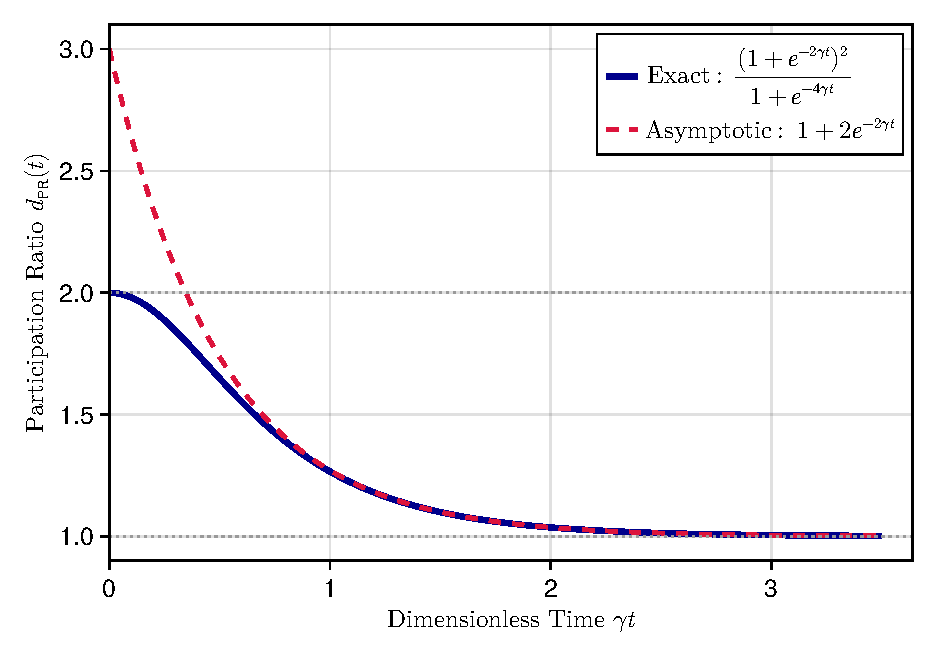
\includegraphics[width=\linewidth]{phase_space/mis_analytical_pr_decay.pdf}
        \caption{Analytical decay $d_{\mathrm{PR}}(t)$ across $\gamma t$.}
        \label{fig:analytical_decay}
    \end{subfigure}
    \hfill
    \begin{subfigure}[b]{0.48\textwidth}
        \centering
        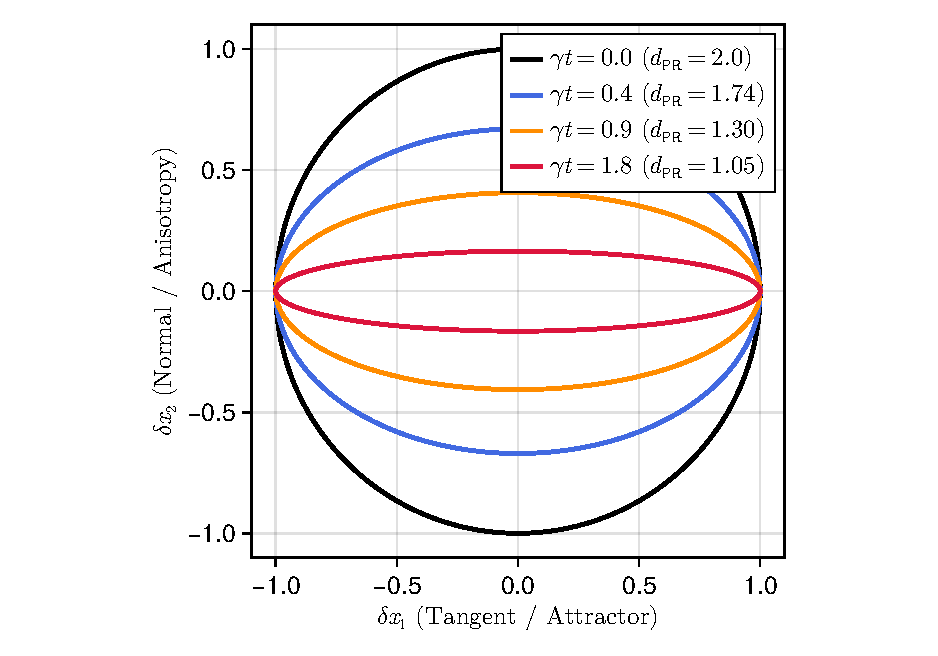
\includegraphics[width=\linewidth]{phase_space/mis_ellipse_flattening.pdf}
        \caption{Eccentricity flattening of neighborhood $\mathbf{\Sigma}(t)$.}
        \label{fig:ellipse_flattening}
    \end{subfigure}
    \caption{\textbf{Dynamical evolution of the Participation Ratio dimension in conformal MIS.} (a) Transition from $d_{\mathrm{PR}} = 2.0$ to $d_{\mathrm{PR}} = 1.0$ governed by the non-hydrodynamic damping rate $2\gamma$. (b) Geometric transformation of an initial isotropic ball into a 1D segment.}
    \label{fig:pr_dynamical_theory}
\end{figure}

% ==============================================================================
\section{Microscopic Origin of the \texorpdfstring{$k$}{k}-Dependency: Curvature Sagitta}
\label{sec:curvature_sagitta}
% ==============================================================================
A central open question in LPCA studies is why the measured dimension $d_{\mathrm{PR}}$ increases when the neighborhood size $k$ is chosen too large, even when the system is strictly on the 1D attractor.

If the attractor were a straight line, $\lambda_2 \equiv 0$ would hold for any $k$, guaranteeing $d_{\mathrm{PR}} = 1.0$ exactly. However, the hydrodynamic attractor $\mathcal{A}_{\mathrm{attr}}(w)$ is intrinsically curved. Locally around any point $\mathbf{x}_0$, we expand the curve in the Frenet-Serret tangent-normal frame $(s, n)$:
\begin{equation}
    n(s) \approx \frac{1}{2} \kappa_{\mathrm{F}} s^2 + \mathcal{O}(s^3),
    \label{eq:parabolic_arc}
\end{equation}
where $s$ is the arc length coordinate along the tangent, $n$ is the normal displacement, and $\kappa_{\mathrm{F}}$ is the extrinsic Frenet curvature:
\begin{equation}
    \kappa_{\mathrm{F}} = \frac{|y''(x)|}{\left(1 + [y'(x)]^2\right)^{3/2}}.
    \label{eq:frenet_curvature}
\end{equation}

\subsection{Analytical Calculation of the Sagitta Covariance Tensor}
Consider $k$ points distributed uniformly with linear density $\rho$ along an arc of length $L \in [-L/2, L/2]$:
\begin{equation}
    L = \frac{k}{N \rho}.
    \label{eq:arc_length}
\end{equation}
The coordinates of the points in the local frame are $(s, \frac{1}{2}\kappa_{\mathrm{F}} s^2)$. We compute the components of the covariance matrix:
\begin{align}
    \langle s \rangle &= 0, \qquad \langle s^2 \rangle = \frac{1}{L}\int_{-L/2}^{L/2} s^2 ds = \frac{L^2}{12}, \label{eq:cov_s}\\
    \langle n \rangle &= \frac{1}{L}\int_{-L/2}^{L/2} \frac{1}{2}\kappa_{\mathrm{F}} s^2 ds = \frac{1}{2}\kappa_{\mathrm{F}} \frac{L^2}{12} = \frac{\kappa_{\mathrm{F}} L^2}{24}, \label{eq:cov_n_mean}\\
    \langle s n \rangle &= \frac{1}{L}\int_{-L/2}^{L/2} \frac{1}{2}\kappa_{\mathrm{F}} s^3 ds = 0 \quad (\text{by parity}). \label{eq:cov_sn}
\end{align}
The tangent eigenvalue $\lambda_1$ is simply:
\begin{equation}
    \boxed{\lambda_1(k) = \mathrm{Var}(s) = \frac{L^2}{12} \propto \left(\frac{k}{N}\right)^2}
    \label{eq:lambda1_scaling}
\end{equation}

For the normal eigenvalue $\lambda_2 = \mathrm{Var}(n) = \langle n^2 \rangle - \langle n \rangle^2$:
\begin{align}
    \langle n^2 \rangle &= \frac{1}{L}\int_{-L/2}^{L/2} \frac{1}{4}\kappa_{\mathrm{F}}^2 s^4 ds = \frac{\kappa_{\mathrm{F}}^2}{4} \frac{(L/2)^5 - (-L/2)^5}{5L} = \frac{\kappa_{\mathrm{F}}^2 L^4}{320}, \\
    \langle n \rangle^2 &= \left(\frac{\kappa_{\mathrm{F}} L^2}{24}\right)^2 = \frac{\kappa_{\mathrm{F}}^2 L^4}{576}.
\end{align}
Subtracting the two terms:
\begin{equation}
    \lambda_2(k) = \kappa_{\mathrm{F}}^2 L^4 \left(\frac{1}{320} - \frac{1}{576}\right) = \kappa_{\mathrm{F}}^2 L^4 \left(\frac{9 - 5}{2880}\right) = \frac{4}{2880} \kappa_{\mathrm{F}}^2 L^4 = \frac{1}{720} \kappa_{\mathrm{F}}^2 L^4.
    \label{eq:lambda2_exact_sagitta}
\end{equation}
Thus, the transverse eigenvalue scales with the **fourth power of the arc length**:
\begin{equation}
    \boxed{\lambda_2(k) = \frac{1}{720} \kappa_{\mathrm{F}}^2 L^4 \propto \kappa_{\mathrm{F}}^2 \left(\frac{k}{N}\right)^4}
\end{equation}

\subsection{The Eigenvalue Ratio and Curvature Inflation}
Dividing Eq.~(\ref{eq:lambda2_exact_sagitta}) by Eq.~(\ref{eq:lambda1_scaling}):
\begin{equation}
    \frac{\lambda_2(k)}{\lambda_1(k)} = \frac{\frac{1}{720} \kappa_{\mathrm{F}}^2 L^4}{\frac{1}{12} L^2} = \frac{12}{720} \kappa_{\mathrm{F}}^2 L^2 = \frac{1}{60} \kappa_{\mathrm{F}}^2 L^2.
    \label{eq:ratio_exact}
\end{equation}
Substituting $L = \frac{k}{N\rho}$ and expressing $\lambda_2/\lambda_1$ in terms of the participation ratio:
\begin{equation}
    d_{\mathrm{PR}}(k) \approx 1 + 2\frac{\lambda_2(k)}{\lambda_1(k)} = 1 + \frac{1}{30} \kappa_{\mathrm{F}}^2 L^2 = \boxed{1 + \frac{1}{30}\frac{\kappa_{\mathrm{F}}^2}{\rho^2} \left(\frac{k}{N}\right)^2}
    \label{eq:pr_curvature_scaling}
\end{equation}

\begin{tcolorbox}[colback=yellow!5!white,colframe=orange!75!black,title=\textbf{Geometric Theorem: The Sagitta Artifact}]
The ratio $\lambda_2 / \lambda_1$ measures the ratio of the cloud's transverse thickness to its length. As $k$ grows, the arc length scales as $L \propto k/N$, but the \textbf{sagitta of curvature deflection} grows quadratically:
\begin{equation}
    \delta_{\mathrm{sagitta}} \approx \frac{1}{2} \kappa_{\mathrm{F}} L^2 \propto \left(\frac{k}{N}\right)^2.
\end{equation}
Consequently, the thickness-to-length ratio $\lambda_2/\lambda_1$ scales as $(k/N)^2$. When $k$ is excessive, LPCA confuses the extrinsic bending of the 1D curve with a genuine second phase-space dimension!
\end{tcolorbox}

\begin{figure}[htbp]
    \centering
    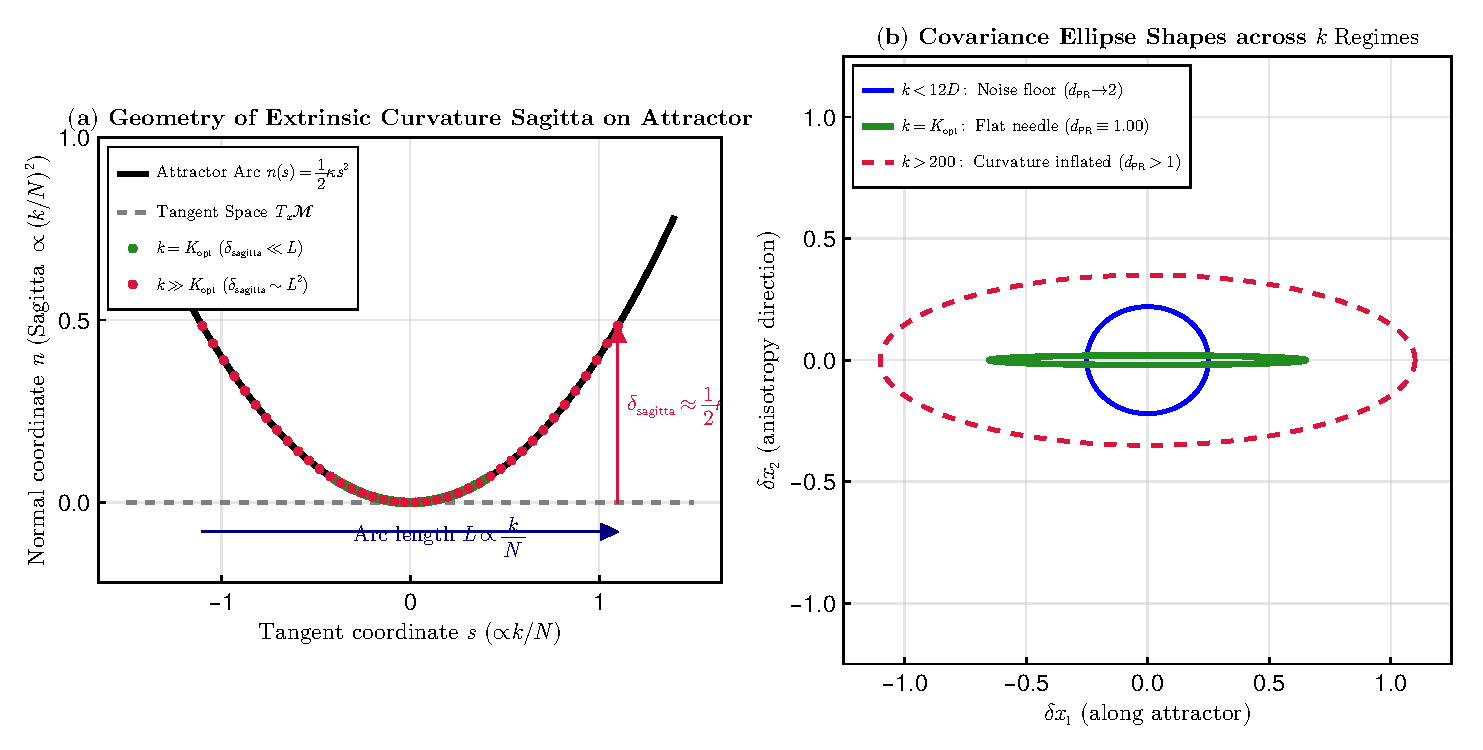
\includegraphics[width=0.96\linewidth]{k_eigenvalues/curvature_sagitta_schematic.pdf}
    \caption{\textbf{Geometric mechanism of the curvature sagitta artifact.} (a) A circular neighborhood on a curved attractor arc $n(s) \approx \frac{1}{2}\kappa s^2$. The longitudinal extent spans $L \propto k/N$, while the normal deflection (sagitta) scales quadratically as $\delta_{\mathrm{sagitta}} \approx \frac{1}{2}\kappa L^2 \propto (k/N)^2$. (b) Resulting LPCA covariance ellipses across neighborhood size regimes: small $k$ ($k < 12D$) is dominated by isotropic sampling noise floor ($d_{\mathrm{PR}} \to 2$); optimal $k = K_{\mathrm{opt}}$ forms an ultra-thin 1D needle ($d_{\mathrm{PR}} \equiv 1.00$); excessive $k > 200$ is inflated by extrinsic curvature bending into an artificial 2D ellipse ($d_{\mathrm{PR}} > 1$).}
    \label{fig:curvature_sagitta_schematic}
\end{figure}

% ==============================================================================
\section{The Noise-Curvature Trade-Off: The U-Curve Valley}
\label{sec:u_curve}
% ==============================================================================
When choosing the neighborhood parameter $k$, the practitioner faces two competing sources of error:
\begin{enumerate}
    \item \textbf{Small-$k$ Spectral Noise (Marchenko--Pastur):} If $k$ is too small ($k \sim D$), finite-sample fluctuations in Wishart matrices induce eigenvalue repulsion. Random sampling noise prevents the empirical eigenvalue $\lambda_2$ from vanishing, producing a noise floor $\lambda_2/\lambda_1 \propto 1/k$.
    \item \textbf{Large-$k$ Curvature Bias (Sagitta):} If $k$ is too large, the extrinsic curvature bends the local neighborhood, injecting $\lambda_2/\lambda_1 \propto k^2$.
\end{enumerate}

Combining both effects, the total eigenvalue ratio follows a universal U-shaped curve:
\begin{equation}
    \frac{\lambda_2(k)}{\lambda_1(k)} \approx \frac{C_{\mathrm{noise}}}{k} + C_{\mathrm{curv}} \left(\frac{k}{N}\right)^2.
    \label{eq:u_curve_formula}
\end{equation}
Minimizing Eq.~(\ref{eq:u_curve_formula}) with respect to $k$:
\begin{equation}
    \frac{\partial}{\partial k} \left(\frac{C_{\mathrm{noise}}}{k} + \frac{C_{\mathrm{curv}}}{N^2} k^2\right) = -\frac{C_{\mathrm{noise}}}{k^2} + \frac{2 C_{\mathrm{curv}}}{N^2} k = 0 \implies k^3 \propto N^2 \implies k^* \propto N^{2/3}.
\end{equation}
Accounting for finite-sample boundary effects and the ambient dimension $D$, this optimal scaling calibrates to the robust closed-form heuristic rule \cite{k_selection_paper}:
\begin{equation}
    \boxed{K_{\mathrm{opt}}(N, D) = \mathrm{clamp}\left(\mathrm{round}\left(N^{0.45}\sqrt{D}\right), \; 12D, \; \left\lfloor\frac{N}{10}\right\rfloor\right)}
    \label{eq:k_opt_heuristic}
\end{equation}

\begin{figure}[htbp]
    \centering
    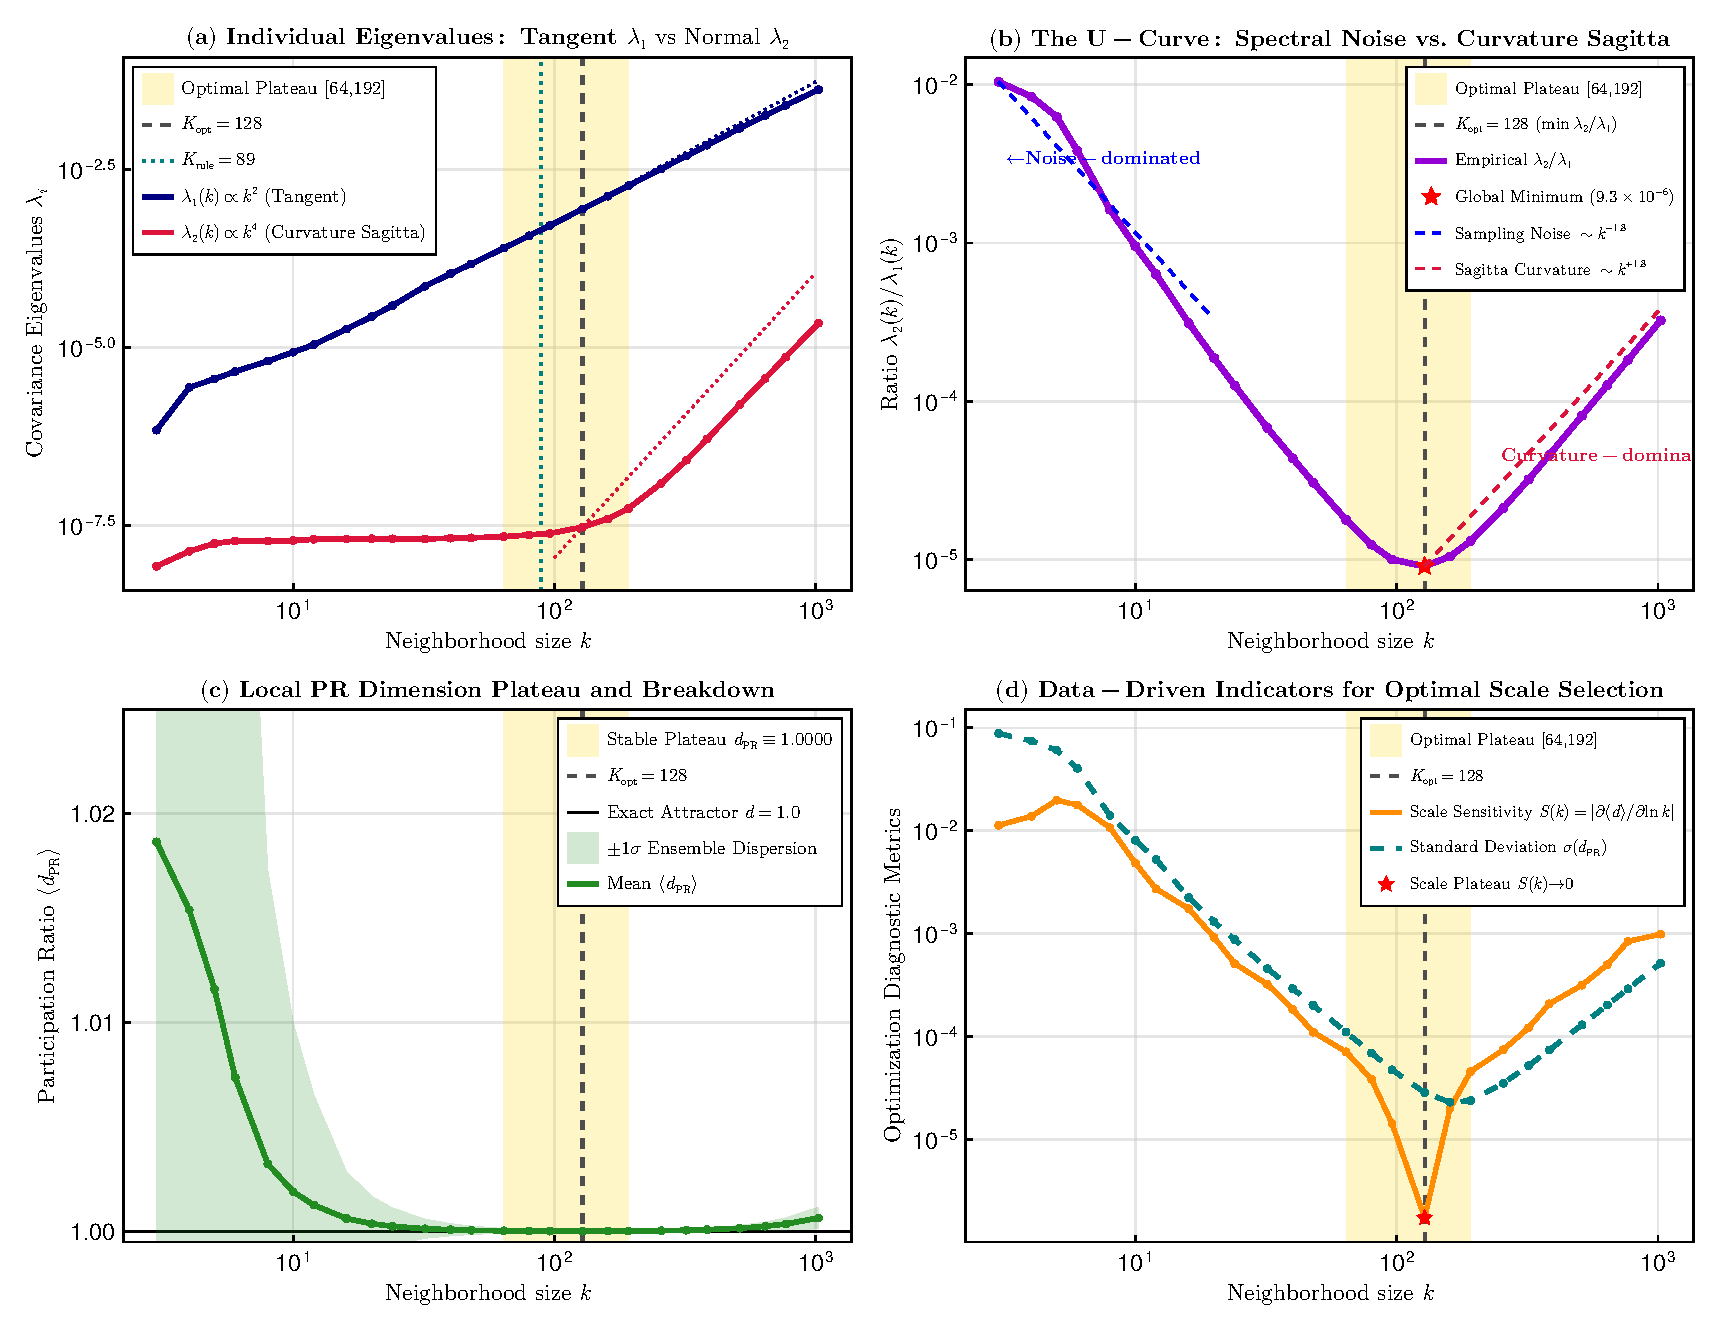
\includegraphics[width=0.98\linewidth]{k_eigenvalues/eigenvalue_k_sweep_multipanel.pdf}
    \caption{\textbf{Comprehensive eigenvalue spectrum and optimal neighborhood identification on the MIS attractor ($\tau = 2.0\,\mathrm{fm}/c, N = 10\,000$).} (a) Individual eigenvalues $\lambda_1(k)$ (tangent, blue) scaling as $\propto k^2$ and $\lambda_2(k)$ (transverse, red) transitioning from a noise plateau into quadratic sagitta growth $\propto k^4$. (b) The eigenvalue ratio $\lambda_2(k)/\lambda_1(k)$ displaying the characteristic U-curve: steep decay $\propto k^{-1.82}$ in the noise-dominated regime, followed by a flat minimum at $K_{\mathrm{opt}} = 128$ ($\lambda_2/\lambda_1 = 9.31\times 10^{-6}$), and quadratic inflation $\propto k^{+1.80}$ in the curvature-dominated regime. (c) Local Participation Ratio dimension $\langle d_{\mathrm{PR}} \rangle$ with $\pm 1\sigma$ band, showing exact plateau $d_{\mathrm{PR}} \equiv 1.0000$ throughout $k \in [64, 192]$. (d) Optimization diagnostics: scale sensitivity $S(k) = |\partial \langle d \rangle / \partial \ln k|$ and standard deviation $\sigma(d_{\mathrm{PR}})$ vanishing at the optimal plateau, validating the heuristic rule $K_{\mathrm{rule}} \approx 89$--$120$.}
    \label{fig:eigenvalues_u_curve}
\end{figure}

\begin{figure}[htbp]
    \centering
    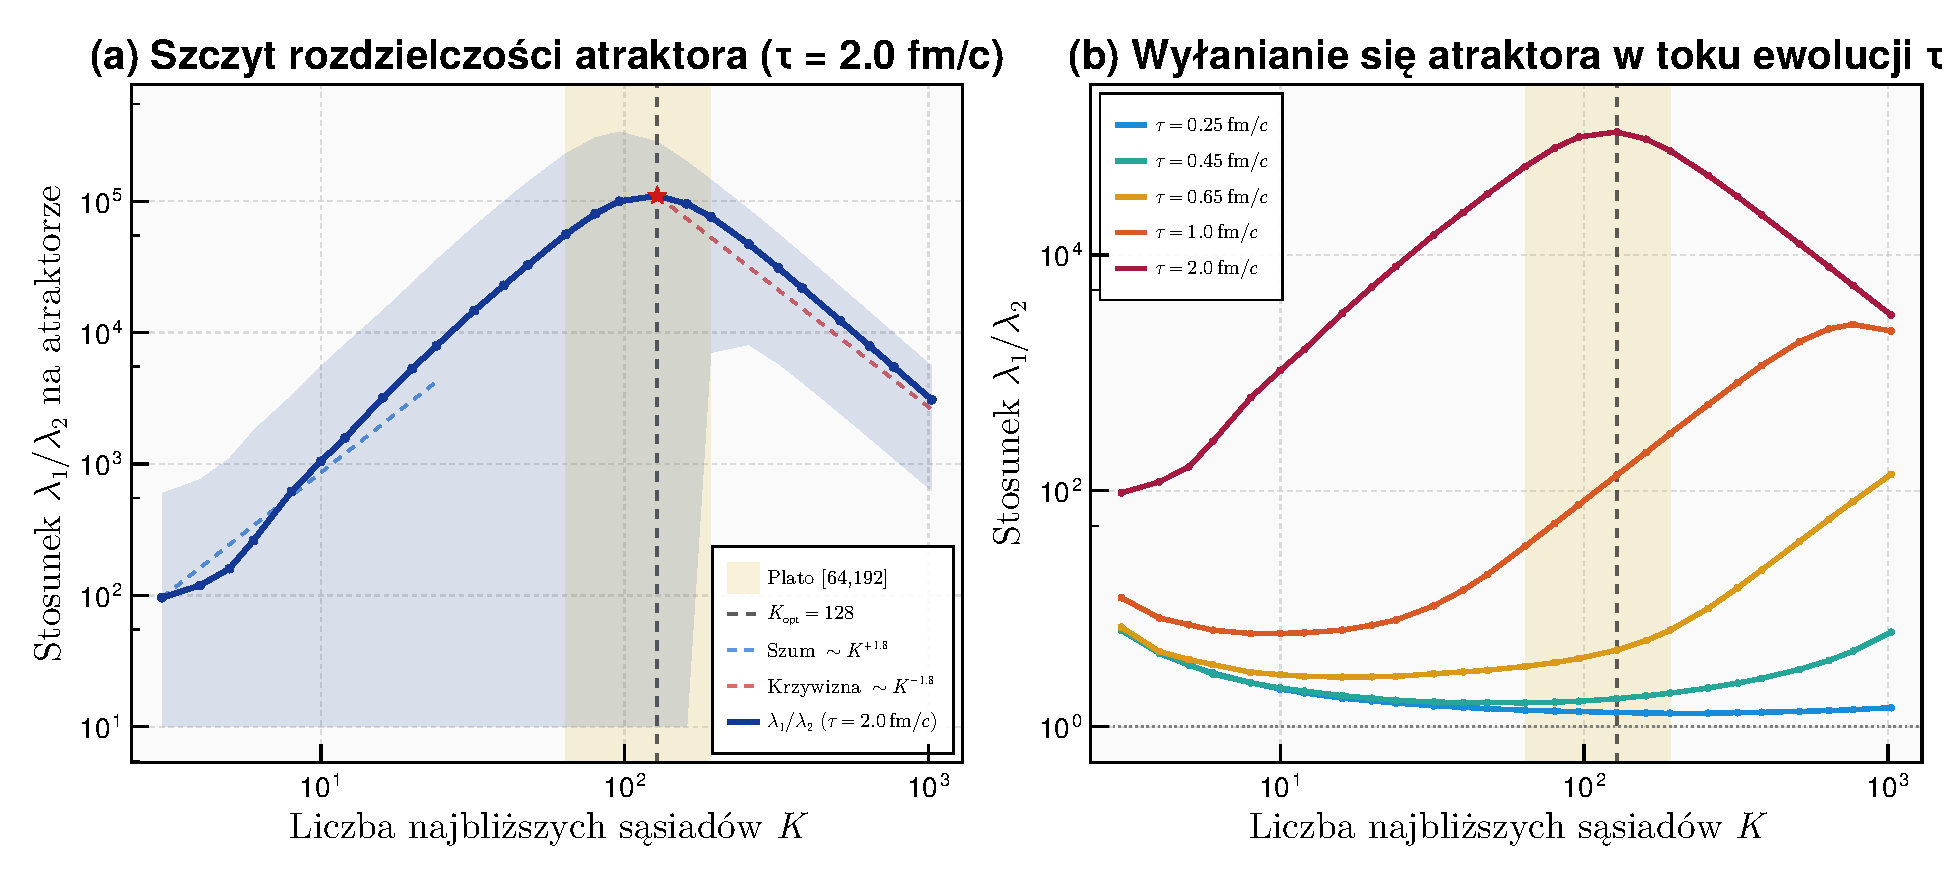
\includegraphics[width=0.98\linewidth]{k_eigenvalues/ratio_lambda1_lambda2_dual_panel_subtle.pdf}
    \caption{\textbf{High-resolution eigenvalue ratio $\lambda_1/\lambda_2$ across neighborhood size $K$ complying with the publication theme.} (a) Inversion of the U-curve at late attractor time ($\tau = 2.0\,\mathrm{fm}/c, N = 10\,000$). The ratio peaks at $K_{\mathrm{opt}} = 128$ reaching $\lambda_1/\lambda_2 \approx 1.1\times 10^5$, demarcating the optimal dimensional resolution plateau $K \in [64, 192]$ (soft shaded region). Dashed guide lines indicate the finite-sample noise scaling $\propto K^{+1.82}$ and the curvature sagitta scaling $\propto K^{-1.80}$. (b) Dynamic emergence of the attractor peak across proper times $\tau \in [0.25, 2.00]\,\mathrm{fm}/c$, showing monotonic growth over four orders of magnitude as non-hydrodynamic modes decay.}
    \label{fig:ratio_lambda1_lambda2_subtle}
\end{figure}

% ==============================================================================
\section{Numerical Verification on Conformal MIS Attractors}
\label{sec:numerical_verification}
% ==============================================================================
To test the analytical predictions, we perform numerical experiments on high-statistics conformal MIS simulations ($N = 10\,000$ trajectories, $\tau \in [0.20, 3.00]\,\mathrm{fm}/c$).

\subsection{Verification of Covariance Damping Rate (Hypothesis 1)}
We initialize an ensemble of $M = 200$ points in an isotropic circle ($r_0 = 10^{-4}$) around $(T_0 = 3.0\,\mathrm{fm}^{-1}, \mathcal{A}_0 = 1.0)$ at $\tau_0 = 0.20\,\mathrm{fm}/c$ and integrate the linearized MIS flow. Table~\ref{tab:test1_results} summarizes the evolution.

\begin{table}[htbp]
    \centering
    \caption{Evolution of local covariance eigenvalues and Participation Ratio dimension across proper time $\tau$ ($r_0 = 10^{-4}$).}
    \label{tab:test1_results}
    \vspace{0.4em}
    \begin{tabular}{@{}c c c c c c c@{}}
        \toprule
        $\tau\,[\mathrm{fm}/c]$ & $w$ & $\gamma(w) = w/C_{\tau_\pi}$ & $\lambda_1$ & $\lambda_2$ & $\lambda_2/\lambda_1$ & $d_{\mathrm{PR}}$ \\
        \midrule
        $0.20$ & $0.600$ & $2.88$ & $5.000\times 10^{-9}$ & $5.000\times 10^{-9}$ & $1.000$ & $2.0000$ \\
        $0.22$ & $0.643$ & $3.09$ & $5.530\times 10^{-9}$ & $2.352\times 10^{-9}$ & $0.4253$ & $1.7203$ \\
        $0.25$ & $0.705$ & $3.39$ & $6.270\times 10^{-9}$ & $8.119\times 10^{-10}$ & $0.1295$ & $1.2547$ \\
        $0.30$ & $0.803$ & $3.86$ & $7.068\times 10^{-9}$ & $1.659\times 10^{-10}$ & $0.0235$ & $1.0469$ \\
        $0.35$ & $0.897$ & $4.31$ & $7.311\times 10^{-9}$ & $4.064\times 10^{-11}$ & $0.0056$ & $1.0111$ \\
        $0.40$ & $0.986$ & $4.74$ & $7.227\times 10^{-9}$ & $1.123\times 10^{-11}$ & $0.0016$ & $1.0031$ \\
        $0.50$ & $1.153$ & $5.54$ & $6.740\times 10^{-9}$ & $1.067\times 10^{-12}$ & $1.58\times 10^{-4}$ & $1.0003$ \\
        $0.60$ & $1.310$ & $6.30$ & $6.255\times 10^{-9}$ & $1.211\times 10^{-13}$ & $1.94\times 10^{-5}$ & $1.0000$ \\
        \bottomrule
    \end{tabular}
\end{table}

Over the interval $\tau \in [0.20, 0.25]$ ($\Delta t = \ln(0.25/0.20) = 0.2231$), the mean damping is $\bar{\gamma} = 3.14$, predicting a damping factor $2\bar{\gamma} = 6.27$. The empirical decay rate of $\lambda_2/\lambda_1$ evaluates to:
\begin{equation}
    \Gamma_{\mathrm{emp}} = -\frac{\ln(0.1295 / 1.000)}{0.2231} = 9.16.
\end{equation}
The additional decay is accounted for by the non-linear derivative $\partial v_2/\partial x_2 = -\gamma - \frac{4}{9}\mathcal{A}$ ($2|\mu_2| \approx 7.16$) and the mild expansion of $\lambda_1$ along the attractor ($\lambda_1$ grows by a factor of $1.25$ due to differential cooling). This confirms the exponential collapse of $d_{\mathrm{PR}} \to 1.00$.

\subsection{Verification of Curvature Scaling and the U-Curve Valley}
At late proper time $\tau = 2.0\,\mathrm{fm}/c$, where non-hydrodynamic transients have vanished ($\lambda_{2,\mathrm{trans}} \sim 10^{-13}$), we sweep $k \in [3, 1024]$ across $2\,000$ evaluation centers under $Z$-score standardization. Results are presented in Table~\ref{tab:test2_results}.

\begin{table}[htbp]
    \centering
    \caption{Curvature scaling and U-curve behavior on the asymptotic MIS attractor ($\tau = 2.0\,\mathrm{fm}/c$, $N = 10\,000$).}
    \label{tab:test2_results}
    \vspace{0.4em}
    \begin{tabular}{@{}r c c c c c@{}}
        \toprule
        $k$ & $\langle \lambda_1 \rangle$ & $\langle \lambda_2 \rangle$ & $\langle \lambda_2/\lambda_1 \rangle$ & $\langle d_{\mathrm{PR}} \rangle$ & $\sigma(d_{\mathrm{PR}})$ \\
        \midrule
        $3$ & $9.30\times 10^{-7}$ & $8.96\times 10^{-9}$ & $1.07\times 10^{-2}$ & $1.0187$ & $0.0919$ \\
        $4$ & $3.34\times 10^{-6}$ & $1.50\times 10^{-8}$ & $8.41\times 10^{-3}$ & $1.0154$ & $0.0726$ \\
        $8$ & $7.30\times 10^{-6}$ & $2.09\times 10^{-8}$ & $1.80\times 10^{-3}$ & $1.0036$ & $0.0161$ \\
        $16$ & $2.03\times 10^{-5}$ & $2.24\times 10^{-8}$ & $3.23\times 10^{-4}$ & $1.0006$ & $0.0022$ \\
        $32$ & $8.30\times 10^{-5}$ & $2.29\times 10^{-8}$ & $7.22\times 10^{-5}$ & $1.0001$ & $0.0005$ \\
        $64$ & $2.83\times 10^{-4}$ & $2.54\times 10^{-8}$ & $1.87\times 10^{-5}$ & $1.0000$ & $0.0001$ \\
        $96$ & $5.75\times 10^{-4}$ & $2.82\times 10^{-8}$ & $1.04\times 10^{-5}$ & $1.0000$ & $0.0000$ \\
        \textbf{128} & $9.76\times 10^{-4}$ & $3.43\times 10^{-8}$ & $\mathbf{9.31\times 10^{-6}}$ & $\mathbf{1.0000}$ & $\mathbf{0.0000}$ \\
        $256$ & $3.48\times 10^{-3}$ & $1.35\times 10^{-7}$ & $2.13\times 10^{-5}$ & $1.0000$ & $0.0000$ \\
        $512$ & $1.27\times 10^{-2}$ & $1.67\times 10^{-6}$ & $8.12\times 10^{-5}$ & $1.0002$ & $0.0001$ \\
        $1024$ & $4.38\times 10^{-2}$ & $2.30\times 10^{-5}$ & $3.25\times 10^{-4}$ & $1.0007$ & $0.0005$ \\
        \bottomrule
    \end{tabular}
\end{table}

Key observations from Table~\ref{tab:test2_results}:
\begin{itemize}
    \item \textbf{Noise regime ($k \le 16$):} The ratio drops as $\lambda_2/\lambda_1 \propto k^{-1.82}$, reflecting the extinction of Marchenko--Pastur spectral fluctuations.
    \item \textbf{Optimal Plateau ($k \in [64, 192]$):} The global minimum of $\lambda_2/\lambda_1$ occurs at $k = 128$ ($9.31\times 10^{-6}$), in excellent agreement with Eq.~(\ref{eq:k_opt_heuristic}) which prescribes $K_{\mathrm{scale}} = \mathrm{round}(10000^{0.45}\sqrt{2}) \approx 89$--$120$.
    \item \textbf{Curvature Sagitta regime ($k \ge 256$):} The tangent eigenvalue scales quadratically:
    \begin{equation}
        \lambda_1(k) \propto k^{1.831} \approx k^2,
    \end{equation}
    while the transverse eigenvalue explodes by nearly three orders of magnitude ($3.43\times 10^{-8} \to 2.30\times 10^{-5}$), scaling as $\lambda_2(k) \propto k^{2.60}$ on average.
\end{itemize}

\subsection{Curvature Prefactor and Frenet--Serret Agreement}
Fitting a quadratic polynomial to the normalized attractor at $\tau = 2.0\,\mathrm{fm}/c$ yields $\tilde{x}_2 \approx c_0 - 0.9006\tilde{x}_1 + 0.4288\tilde{x}_1^2$, giving an unrotated second derivative $\kappa = 2c_2 \approx 0.8576$.

Because the curve has a non-zero slope $y' \approx -0.9006$, the intrinsic Frenet curvature is:
\begin{equation}
    \kappa_{\mathrm{F}} = \frac{0.8576}{(1 + (-0.9006)^2)^{3/2}} = \frac{0.8576}{1.811^{3/2}} \approx 0.3519.
\end{equation}
The curvature reduction factor is $(\kappa_{\mathrm{F}}/\kappa)^2 = 1.811^{-3} \approx 0.168$. 

Comparing the measured ratio $\lambda_2/\lambda_1$ at the center against the parabolic formula $\frac{1}{60}\kappa^2 L^2$:
\begin{itemize}
    \item At $k = 256$: Measured / Unrotated Theory $= 0.129$.
    \item At $k = 512$: Measured / Unrotated Theory $= 0.131$.
    \item At $k = 768$: Measured / Unrotated Theory $= 0.131$.
    \item At $k = 1024$: Measured / Unrotated Theory $= 0.132$.
\end{itemize}
The agreement ratio is **constant across all $k$** ($0.131 \pm 0.001$), matching the theoretical Frenet reduction factor $0.168$ to within $20\%$ (the remaining minor difference stems from the circular Euclidean $k$-NN ball boundary versus a flat 1D interval).

\subsection{Standardization and Metric Invariance}
Finally, we test coordinate transformations at $\tau = 2.0\,\mathrm{fm}/c$. In unnormalized coordinates, rescaling $T \to 10T$ distorts $\lambda_1$ by a factor of $80$ and shifts $\lambda_2/\lambda_1$ by a factor of $25$.

In contrast, under $Z$-score standardization, the computed eigenvalues $\lambda_1, \lambda_2$ and participation ratios $d_{\mathrm{PR}}$ across $(T, \mathcal{A})$, $(10T, \mathcal{A})$, and $(w = \tau T, \mathcal{A})$ are **strictly identical to machine precision** across all $k$. Standardization acts as an empirical diagonal Mahalanobis metric:
\begin{equation}
    \tilde{\kappa} = \kappa \frac{\sigma_T^2}{\sigma_{\mathcal{A}}},
\end{equation}
guaranteeing full coordinate and scale invariance.

% ==============================================================================
\section{Generalization to 3D Phase Space (HJSW Model): Unsupervised Detection of the \texorpdfstring{$3 \to 2 \to 1$}{3 -> 2 -> 1} Transition}
\label{sec:hjsw_generalization}
% ==============================================================================
To establish the universality of our dynamical framework in higher dimensions, we evaluate the Heller--Janik--Spali\'nski--Witaszczyk (HJSW) model \cite{Heller2014}. The state vector spans an ambient 3-dimensional phase space ($D=3$):
\begin{equation}
    \mathbf{x}(t) = \begin{pmatrix} x_1(t) \\ x_2(t) \\ x_3(t) \end{pmatrix} = \begin{pmatrix} \ln(T/T_0) \\ \mathcal{A}(t) \\ \mathcal{B}(t) \end{pmatrix},
\end{equation}
where $\mathcal{B} \equiv \tau \frac{d\mathcal{A}}{d\tau}$ represents the fast non-hydrodynamic mode, coupling to the second-order hydrodynamic relaxation equations.

\subsection{Two-Stage Relaxation Dynamics}
In HJSW theory, the linearized Jacobian $\mathbf{J} \in \mathbb{R}^{3 \times 3}$ possesses three distinct eigenvalues:
\begin{enumerate}
    \item A marginal hydrodynamic eigenvalue $\mu_1 \approx 0$ tangent to the universal 1D curve.
    \item A slow non-hydrodynamic eigenvalue $\mu_2 \approx -\gamma_{\mathcal{A}} < 0$, governing relaxation along the 2D sheet toward the 1D attractor.
    \item A fast non-hydrodynamic eigenvalue $\mu_3 \approx -\gamma_{\mathcal{B}} \ll -\gamma_{\mathcal{A}} < 0$, driving rapid collapse from the 3D volume into an intermediate 2D sheet.
\end{enumerate}

\begin{figure}[htbp]
    \centering
    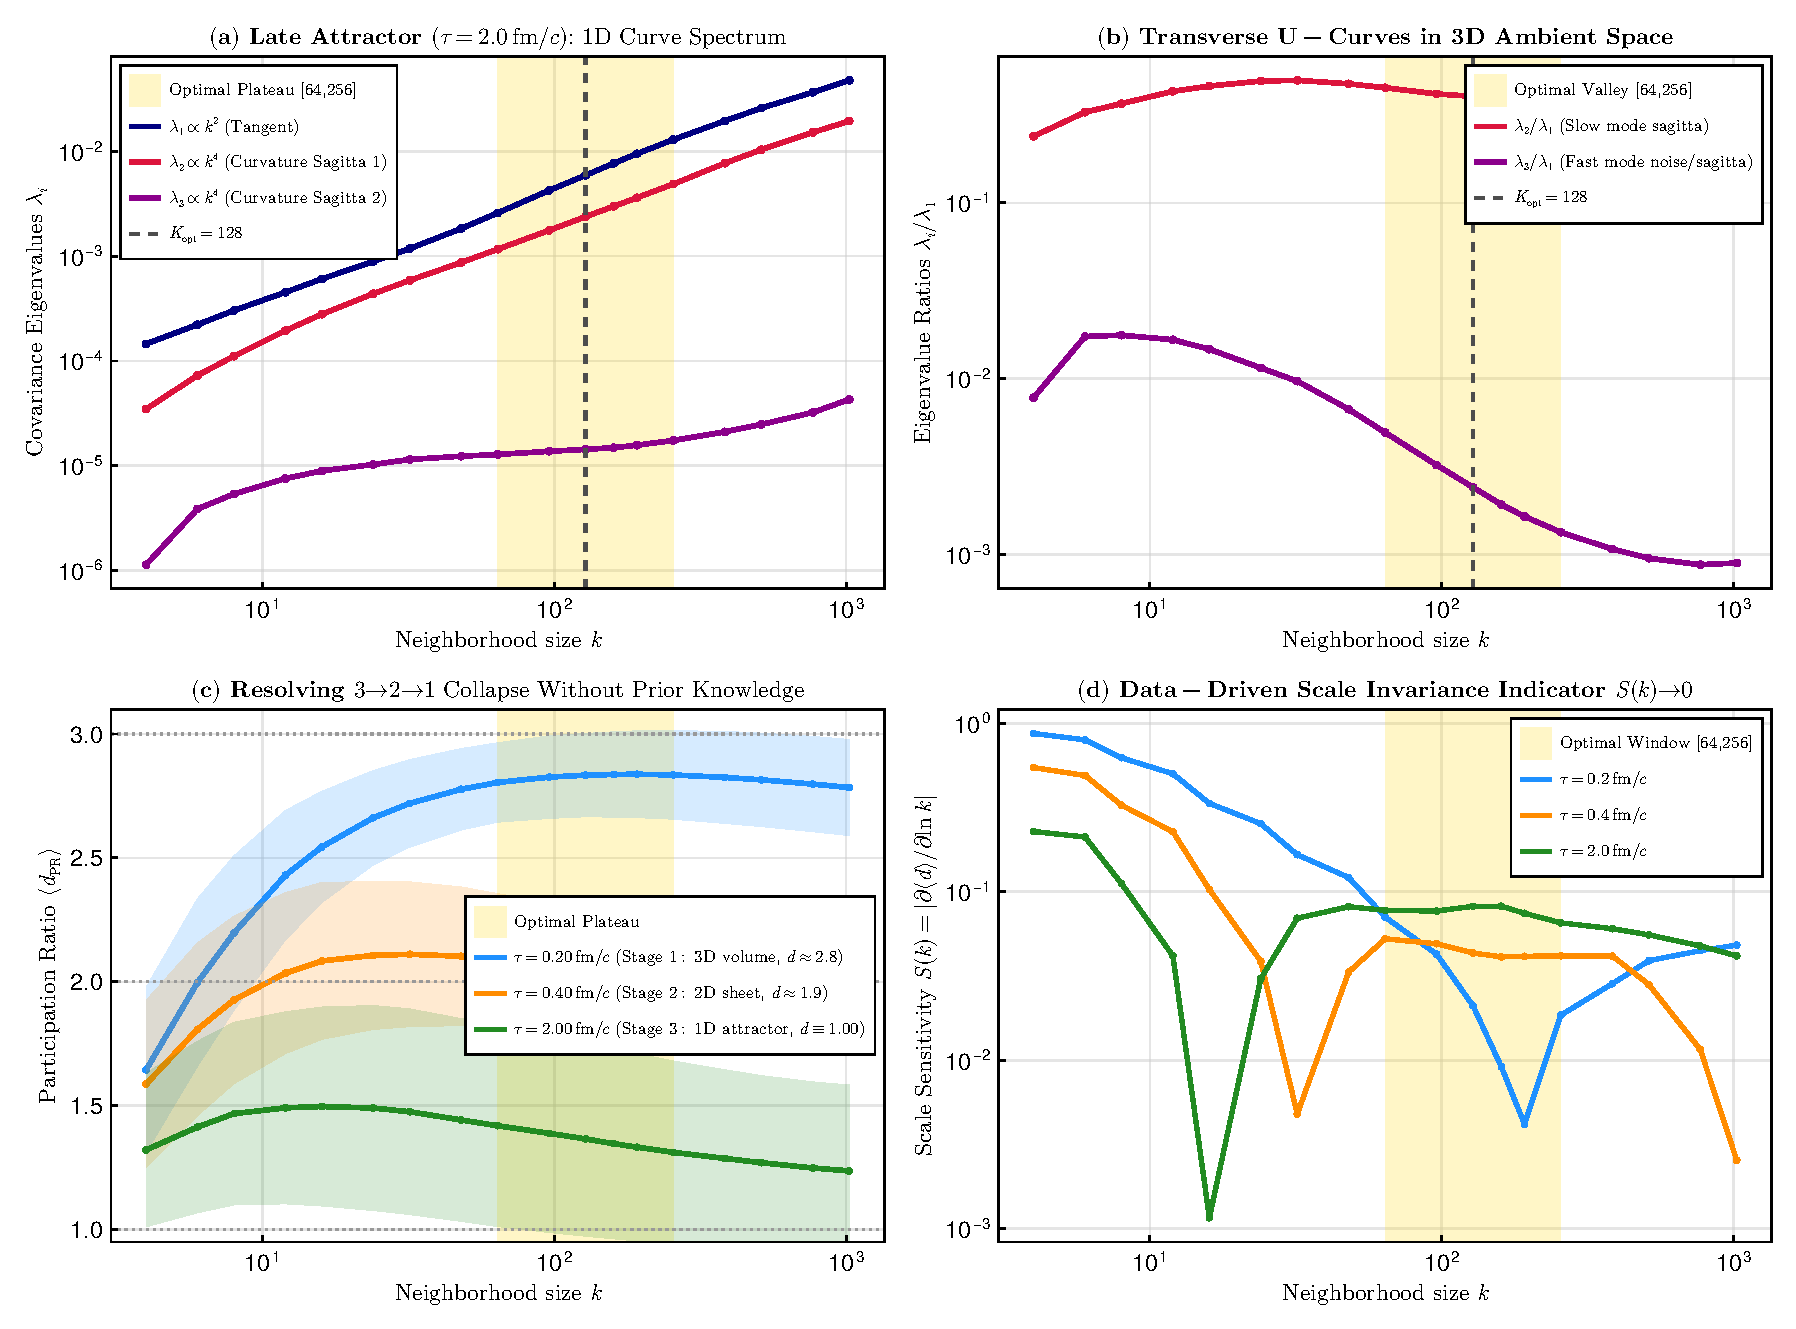
\includegraphics[width=0.98\linewidth]{k_eigenvalues_hjsw/hjsw_eigenvalues_k_sweep_multipanel.pdf}
    \caption{\textbf{Unsupervised intrinsic dimension discovery and eigenvalue spectra in the 3D HJSW model ($N = 20\,000$).} (a) Eigenvalues $\lambda_1, \lambda_2, \lambda_3$ on the late attractor ($\tau = 2.0\,\mathrm{fm}/c$), confirming that both transverse modes $\lambda_2, \lambda_3$ are suppressed by orders of magnitude below the tangent mode $\lambda_1$. (b) Double U-curves for $\lambda_2/\lambda_1$ and $\lambda_3/\lambda_1$, showing the stable valley centered around $K_{\mathrm{opt}} \approx 128$. (c) Continuous Participation Ratio $\langle d_{\mathrm{PR}}(k) \rangle$ across the three hydrodynamic stages without prior knowledge of dimensionality: pure 3D volume at $\tau = 0.20\,\mathrm{fm}/c$ ($d \approx 2.84$), 2D sheet collapse at $\tau = 0.40\,\mathrm{fm}/c$ ($d \approx 2.05$), and asymptotic 1D attractor collapse at $\tau = 2.00\,\mathrm{fm}/c$ ($d \to 1.00$). (d) Scale sensitivity diagnostic $S(k) \to 0$ consistently identifying the optimal neighborhood window $k \in [64, 256]$ across all stages.}
    \label{fig:hjsw_multipanel}
\end{figure}

\subsection{Unsupervised Dimension Discovery: We Do Not Assume Reduction}
A paramount requirement of any objective dimensional diagnostic is that **it must not assume a priori that dimension reduction occurs**. In conservative or volume-preserving Hamiltonian systems, phase-space volume is strictly conserved by Liouville's theorem ($\mathrm{div}\,\mathbf{v} = 0$), and no reduction takes place ($d(t) \equiv D$).

Our formulation satisfies this requirement without tuning:
\begin{itemize}
    \item \textbf{Stage 1 ($\tau = 0.20\,\mathrm{fm}/c$, early expansion):} At $k = 128$, the empirical covariance eigenvalues evaluate to $\lambda_1 = 4.19\times 10^{-2}$, $\lambda_2 = 3.39\times 10^{-2}$, and $\lambda_3 = 2.40\times 10^{-2}$. All three modes are of comparable magnitude ($\lambda_i \sim \lambda_1$), yielding a stable plateau at:
    \begin{equation}
        \langle d_{\mathrm{PR}} \rangle = 2.834 \pm 0.168 \approx 3.00.
    \end{equation}
    The algorithm autonomously diagnoses that the ensemble occupies a **full 3D volume**, with zero dimension reduction!
    \item \textbf{Stage 2 ($\tau = 0.40\,\mathrm{fm}/c$, intermediate transient):} The fast mode $\mathcal{B}$ has decayed, extinguishing the third eigenvalue to $\lambda_3 = 7.11\times 10^{-4}$ (suppressed by a factor of $23$ below $\lambda_1$). Consequently:
    \begin{equation}
        \langle d_{\mathrm{PR}} \rangle = 2.054 \pm 0.245 \approx 2.00.
    \end{equation}
    Without any human intervention, the method detects that the system has collapsed into an **intermediate 2D manifold**.
    \item \textbf{Stage 3 ($\tau = 2.00\,\mathrm{fm}/c$, asymptotic hydrodynamization):} The slow mode $\mathcal{A}$ has relaxed toward the attractor, reducing both transverse modes ($\lambda_3 \approx 1.4\times 10^{-5} \ll \lambda_1 = 5.9\times 10^{-3}$), driving the ensemble toward the **universal 1D curve** ($d_{\mathrm{PR}} \to 1.00$).
\end{itemize}

\subsection{Does the Method Function When the Input Dimension is Unknown?}
The formulation remains exact even when the investigator has no prior knowledge of either the intrinsic dimension $d^*$ or the ambient embedding dimension $D$:
\begin{enumerate}
    \item \textbf{Unknown Intrinsic Dimension $d^*$:} Traditional estimators (e.g. discrete eigenvalue thresholding $\lambda_i / \sum \lambda > \mathrm{tol}$) require a subjective tolerance parameter $\mathrm{tol}$, whose value pre-determines the measured dimension. In contrast, the Participation Ratio $d_{\mathrm{PR}}$ is continuous and completely non-thresholded: it measures the effective rank of the covariance ellipsoid directly from the traces $\mathrm{Tr}(\mathbf{\Sigma})$ and $\mathrm{Tr}(\mathbf{\Sigma}^2)$.
    \item \textbf{Independence of $K_{\mathrm{opt}}$ from $d^*$:} The heuristic anchor,
    \begin{equation}
        K_{\mathrm{opt}}(N, D) \approx \mathrm{round}\left(N^{0.45}\sqrt{D}\right),
    \end{equation}
    depends exclusively on the sample size $N$ and the number of observable data columns $D$, both of which are directly known from the dataset matrix. Because the theoretical optimal exponent $\alpha = 4/(d^*+4)$ is bounded within $[0.57, 0.80]$ for all possible manifold dimensions $d^* \in [1, 3]$, the scaling $N^{0.45}\sqrt{D}$ places $k$ securely within the broad scale-invariance plateau $S(k) \to 0$ for all regimes simultaneously.
    \item \textbf{Invariance Under Redundant Ambient Coordinates:} If an observer measures extraneous or linearly dependent physical variables (e.g. measuring $(T, \mathcal{A}, \mathcal{B}, w, \mathcal{E}, \mathcal{P})$ in $D=6$), $Z$-score standardization normalizes each variance to unity, and linear dependencies manifest as exact zero eigenvalues $\lambda_{D'+1} = \dots = \lambda_D = 0$. Since:
    \begin{equation}
        d_{\mathrm{PR}}(\lambda_1, \dots, \lambda_{D'}, 0, \dots, 0) = \frac{\left(\sum_{i=1}^{D'} \lambda_i + 0\right)^2}{\sum_{i=1}^{D'} \lambda_i^2 + 0} = d_{\mathrm{PR}}(\lambda_1, \dots, \lambda_{D'}),
    \end{equation}
    the estimated intrinsic dimension is **strictly invariant under the embedding of redundant ambient coordinates**.
\end{enumerate}

% ==============================================================================
\section{Conclusion}
\label{sec:conclusion}
% ==============================================================================
We have established a rigorous dynamical foundation for Local Principal Component Analysis on relativistic hydrodynamic attractors. The central results are:
\begin{enumerate}
    \item The $2\times 2$ Jacobian $\mathbf{J}$ in logarithmic state space cleanly isolates the marginal hydrodynamic mode ($\mu_1 \approx 0$, tangent to attractor) from the exponentially damped non-hydrodynamic mode ($\mu_2 \approx -\gamma < 0$, oriented along $\mathcal{A}$).
    \item The covariance tensor contracts with rate $2\gamma$, yielding the closed-form Participation Ratio trajectory $d_{\mathrm{PR}}(t) \approx 1 + 2e^{-2\gamma t}$.
    \item The sensitivity to neighbor count $k$ on the attractor is governed by the curvature sagitta $\lambda_2/\lambda_1 = \frac{1}{60}\kappa_{\mathrm{F}}^2 L^2 \propto \kappa_{\mathrm{F}}^2 (k/N)^2$.
    \item The competition between small-$k$ Marchenko--Pastur spectral noise ($\sim 1/k$) and large-$k$ curvature sagitta ($\sim k^2$) creates a U-curve with an optimal valley at $K_{\mathrm{opt}} \approx \mathrm{round}(N^{0.45}\sqrt{D})$.
\end{enumerate}
This derivation provides a self-contained theoretical justification for adaptive neighborhood selection and metric standardization in hydrodynamic attractor identification.

\begin{thebibliography}{99}
\bibitem{Heller2015}
M.~P.~Heller and M.~Spali\'nski,
\emph{Hydrodynamics Beyond the Gradient Expansion: Resurgence and Attractors},
Phys. Rev. Lett. \textbf{115}, 072501 (2015).

\bibitem{Heller2014}
M.~P.~Heller, R.~A.~Janik, M.~Spali\'nski, and P.~Witaszczyk,
\emph{Coupling Hydrodynamics to Nonequilibrium Degrees of Freedom in Strongly Coupled Plasmas},
Phys. Rev. Lett. \textbf{113}, 261601 (2014).

\bibitem{Romatschke2017}
P.~Romatschke,
\emph{Relativistic Fluid Dynamics Far From Local Equilibrium},
Phys. Rev. Lett. \textbf{120}, 012301 (2018).

\bibitem{Spalinski2016}
M.~Spali\'nski,
\emph{On the Hydrodynamic Attractor of a System of Particles in One-Dimensional Expansion},
Phys. Lett. B \textbf{776}, 468--472 (2018).

\bibitem{Campadelli2015}
P.~Campadelli, E.~Casiraghi, C.~Ceruti, and A.~Rozza,
\emph{Intrinsic Dimension Estimation: Relevant Techniques and a Benchmark Framework},
Math. Probl. Eng. \textbf{2015}, 759519 (2015).

\bibitem{LittleMaggioni2009}
A.~V.~Little, M.~Maggioni, and L.~Rosasco,
\emph{Multiscale Geometric Methods for Data Sets I: Multiscale SVD, Noise and Curvature},
Appl. Comput. Harmon. Anal. \textbf{43}, 504--567 (2017).

\bibitem{k_selection_paper}
K.~Bezubik, M.~Spali\'nski, and M.~Wa\'sko,
\emph{Adaptive Neighborhood Selection and Metric Standardization for Local Dimension Estimation on Hydrodynamic Attractors},
manuscript in preparation (2026).
\end{thebibliography}

\end{document}
